During our brainstorm sessions it quickly became clear that we needed a policy engine that was flexible. This we deducted from the cases discussed amongst team members. With inspiration from other building management systems (see \ref{chapter:relatedwork}) and looking at the building simulator we had to communicate with, we came up with the concept of policies that consist of two types of overall statements; \textit{if-statements} and \textit{set statements}. If-statements works as if-statements in many popular GPL's, with a condition consisting of expressions, a then-clause and an else-clause. Set statements work by setting a value on the building simulator (in effect it acts as an actuator).

\section{The policy expression language}
Merriam-Webster defines \textit{policy} as; "A definite course or method of action selected from among alternatives and in light of given conditions to guide and determine present and future decisions."

We have defined a policy as a collection of statements operating on sensors and actuators residing in the building simulator. The policy also has a start time and a stop time. It is also possible to de-activate a policy completely - without deleting it entirely.

A statement can either be a SetStatement or an IfStatement. The SetStatement sets an value in the simulator. The backend implementation allows nested If-statements, making the policies both flexible and simple. 

An If-statement can contain multiple expressions that all are being anded when evaluated. If the user wants to make an If-statement with or'ed expressions, she will have to use a nested if. The optimal solution to this would have been to make a safe left-recursive model. We did not have enough time for this, but we will elaborate further on this subject in the discussion (see \ref{sec:product}). 

The statements are organized as a list. Each statement will be executed (set) or evaluated (if) in the order that they are persisted. Each if-statement has two lists that contain the statements belonging to the then-clause and the else-clause.

\section{Architecture}
The system that we have designed consists of four overall parts;
\begin{itemize}
	\item The management website (front end)
	\item The policy engine (back end)
	\item The database for storing policies (back end)
	\item The provided building simulator (back end)
\end{itemize}

Figure \ref{fig:design-system-architecture} illustrates the relationship of the system parts. In terms of MVC the \textit{model} and the \textit{controller} is the servlet containing data and business logic. The servlet reacts to several urls (see Figure~\ref{fig:design-servlet-architecture}), that functions as an interface for an operation needed in the system. The \textit{View} is the rendered html based on JQuery.

\begin{figure}[t]
\center{
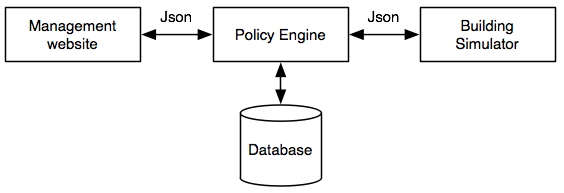
\includegraphics[scale=.5]{chapters/design-system-architecture.png}
\caption{The PolicyEngine system architecture.}\label{fig:design-system-architecture}}
\end{figure}

A statement can either be a SetStatement or an IfStatement. The SetStatement sets an value in the simulator (in effect it is an actuator). The backend implementation allows nested If-statements. If-then-else statements have been around since the early versions of Basic, and is an established way of achieving conditional computer logic. Even though the intended audience of our system is not considered computer experts, the if-then-else concept is easy to understand and catches on fast when interviewing people. An If-statement can contain multiple expressions that all are being anded when evaluated. If the user wants to make an If-statement with or'ed expressions, she will have to use a nested if. This raises the complexity and we do not consider this to be an optimal solution. The optimal solution in this case would have been to make a proper expression language that is left recursion safe, for example based on~\cite{left-recursion}. This would also solve our lacking or's in the condition of the if-statements. Unfortunately we did not realize this until around two thirds into the development. Since our jQuery~\cite{jquery} parsing on the frontend naturally is strongly bound to domain classes on the backend (due to JSon serialization using Gson~\cite{gson}), any big changes at that point would affect both the backend and the frontend. We realized then that it would be too time consuming to change the system. We therefore leave it up to future work, and we elaborate further on this subject in the \nameref{chapter:discussion} (Section~ref{chapter:discussion}). 

\subsection{The management website}
The management website resides is based in a small collection of html pages that relies heavily on JQuery. The building policy administrator opens the main page in a browser, and gets an overview of all the policies and can perform CRUD operations on them.

During the design phase for the GUI of the management website, we used Photoshop sketches that we mailed and transferred via Skype to each other. One from the kenyan team also assisted in this phase. After discussing how to best present policies to the building policy administrator in the time we had available, we choose an indented page layout when presenting the policies. By choosing this type of GUI, as opposed to a more tabular view on the if's, we elected a GUI that is flexible enough to extend to a recursive rendering which clearly matters a greatly when then-clauses can contain other if-statements that again contain then-clauses and so forth. For implementation see Section \ref{chapter:implementation}.

\subsection{The policy engine}
The policy engine consists of a servlet and domain classes for the expression language needed to build policies. The servlet is the core of our policy engine. It has three main objectives;

\begin{figure}[b]
\center{
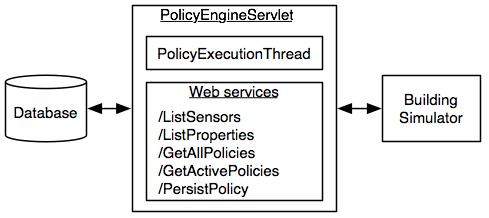
\includegraphics[scale=.5]{chapters/design-servlet-architecture.png}
\caption{A overview model of the PolicyEngineServlet.}\label{fig:design-servlet-architecture}}
\end{figure}

\begin{itemize}
	\item The timed, repetitive execution of policies that currently are active
	\item Serving web service requests to the JQuery front end
	\item Serving the management website html files
\end{itemize}

An overview model of the PolicyEngineServlet can be seen in Figure \ref{fig:design-servlet-architecture}.

As servlet container we use Tomcat 7.0.37. On servlet container startup the servlet will read various configuration values, and then set up a thread that manages the timed, repetitive execution of active policies. While testing the system policies were executed every 5 seconds, but this is configurable. The servlet will start by querying the database for active profiles, which are defined as policies that have a boolean flag (active) set to true, while the current time is within the policie's \textit{from} and \textit{to} time. This will result in a list of policies that should be executed. Then all sensor id values of all if-statements are fetched from the building simulator, and cached in an in-memory datastructure. Thereafter the policies are executed. 

This design was based on several iterations of group discussions. Everyone wanted a solution that worked efficient and fast, within the loosely defined scope that we initially had set for the system development. And clearly, our project should fit in the timeframe allowed for the project.

The first couple of design proposals from some team members were based on SQL integration directly into the database that the building simulator uses. This direct integration could be argued as being a good, although strongly coupled integration. Also, it did not feel like a real world scenario (which we assume is one of the points of this course) if we could access the database directly in this way. Traditionally building systems tend to be closed source proprietary systems with few, if any, integration point. Today there exists different kind of protocols (KNX, LON and BACnet to name a few) that allows some integration to existing building automation systems (for example CTS \footnote{Central Tilstandskontrol- og Styring} systems that are widely used in Denmark). Since our project deals with a building simulator, we do not have to worry about these kind of implementation details --- but we are aware that they are there.

Later design proposal revolved around the idea of having more or less mirrored sensor data in a separate database. Data should be transferred at regular intervals, and the policies should be executed against the copy. This turned out to be a too unsophisticated solution - and the problem to decide which sensor data to mirror remained. Finally we arrived at the rest API integration for fetching and setting values, and our own database to hold the policies and their time information.

\subsection{The database}
The database used is a mySQL 5.5.29 and used for storing the policies. At the moment we only use one table containing all the policies.

\subsection{The building simulator}
The building simulator provided in the course has not been changed or modified in any way.

\subsection{Limitations \& alternatives}
The core functionality of our policy engine is the expression language. During the initial research for scripting languages we looked at several established embeddable scripting languages.

\begin{table}[h]
	\center
	\begin{tabular}{rc}
		\textbf{Name}	&	\textbf{Description}\\
		Jython	&	Python scripting\\
		JRuby	&	Ruby scripting\\
		Tcl/Java	&	Tcl scripting\\
		Rhino	&	Javascript scripting\\
		BSF		&	Bean Scripting Framework*
	\end{tabular}
	\caption{Established scripting languages found during research}\label{tbl:design-scripting-languages}
\end{table}

* The BSF supports several languages.

As stated earlier, we believed that developing our own scripting language was best given the resources we had available and the timespan of the project. It would propose a great number of challenges to integrate one of the scripting languages into our code. We only needed a small subset of the functionality (mainly the if-then-else construct) and we based our decision on developing our own language on the timewise return of investment.

In the team we had some initial discussions if we should use technologies like Xtext~\cite{xtext}, Xbase~\cite{xbase} and EMF~\cite{emf}. Xtext is a framework for developing programming languages and domain specific languages. Xbase is a partial programming language built in Xtext and used for integrating into other programming languages and domain specific languages. Xbase would be able to give us an working expression language. EMF is the Eclipse Modeling Framework, a modeling framework and code generation tool. Some of the team members in the danish group had used those technologies during the ITU course Model Driven Development, but no kenyan team members had any experience with these technologies. This would in effect mean that they would need to acquire the skills learned during Model Driven Development, while simultaneous working and contributing to our joint policy engine project. We deemed this unrealistic. Another argument for not using this set of technologies is that Xbase seemed too daunting a project to undertake due to it's current state. At the time of writing, only 25 questions have been tagged with Xbase on~\cite{stackoverflow} - a website used frequently by the danish team members when in need of coding assistance. The lack of Xbase examples and documentation also reveals that it is a very new, and unfinished, product. Since Xbase would be the caretaker of the expression language, we could have opted to forego just that, and still use Xtext and optionally EMF. We considered this but arrived at the conclusion that using Xtext alone would not give us that much, since our language is small. Also the amount of overhead introduced by using Xtext, both in complexity but also in the generated code, would further add to the confusion of our team members with no experience with this technology. 

Based on the these arguments we chose to develop the functionality ourselves. We also considered that task to be more \textit{fun}! Developing our own scripting language made us think about how languages are designed, and the role of parsers, compilers and interpreters.


\begin{figure}
\center{
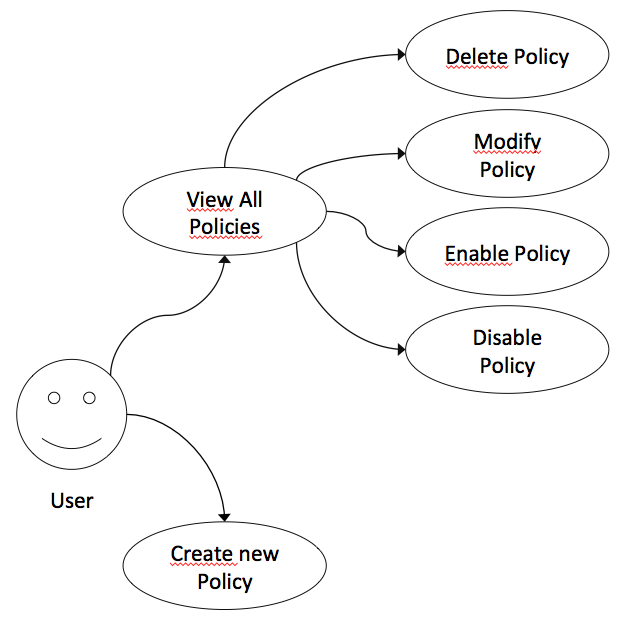
\includegraphics[scale=.5]{use-case-diagram.png}
\caption{Use Case Diagram.}\label{fig:use-case-diagram}}
\end{figure}